\documentclass{article}
\usepackage{mathtools}
\usepackage{listings}
\usepackage{tikz-network}

\begin{document}
\title{CS320 Homework 6}
\author{Dustin Randall}
\maketitle

\section{Show the BFS and DFS traversal of the provided graph, starting from vertex F.}
\subsection{BFS Traversal}
f h d b i n m
\subsection{DFS Traversal}
f h d b n m i

\section{Give the pseudocode for converting a binary tree into an adjacentcy list.}
\subsection{Pseudocode}
I would approach this problem using a BFS traversal of the tree.
Each time we visit a node, we add it's children to the adjacentcy list, and to the queue.
If we know that we're given a complete binary tree, we can early out when we reach a node with no children.
\begin{lstlisting}
    function toAdjList(root) {
        adjList = new List<List<Node>>()
        if(root is null) return

        queue = new Queue(root)
        while(!queue.isEmpty()) {
            current = queue.dequeue()
            adjlist[current] = List<Node>()
            if(current.left is not null) {
                adjList[current].add(current.left)
                queue.enqueue(current.left)
            }
            if(current.right is not null) {
                adjList[current].add(current.right)
                queue.enqueue(current.right)
            }
            // optionally early out here if right is null
        }
        return adjList
    }
\end{lstlisting}
\subsection{Runtime analysis}
The runtime of this algorithm is $O(n)$ because each node is visited exactly once, and the work done is constant for each node.

\section{Design a BFS search using an adjacentcy matrix.}
\subsection{Pseudocode}
Given an adjacentcy matrix, we take the starting point, and find all of it's connected neighbors.
Unfortunately, with an adjacentcy matrix, we have to check every other vertex to see if it's connected or not.
Each connected neighbor gets added to the queue, and the algorithm continues as normal.
\begin{lstlisting}
function BFS(adjMatrix, start) {
    visited = new Set()
    queue = new Queue(start)
    while(!queue.isEmpty()) {
        current = queue.dequeue()
        print(current) // or whatever you're doing in the search
        foreach neighbor in adjMatrix[current] {
            if(neighbor is not null and neighbor not in visited) {
                visited.add(neighbor)
                queue.enqueue(neighbor)
            }
        }
    }
}
\end{lstlisting}

\subsection{Runtime Analysis}
The runtime of this algorithm is now $O(V^2)$ because for each vertex, we need to check every other vertex to see if it's connected or not.
In an adjacentcy list implementation, the runtime is $O(V + E)$ which could be $O(V^2)$ in a dense graph, but is often much better.

\section{Provide a non-recursion based DFS}
I've seen someone change from BFS to DFS by changing just a single character, but I'll simply use a stack instead of a queue.
\begin{lstlisting}
function DFS(adjList, start) {
    visited = new Set()
    stack = new Stack(start)
    while(!stack.isEmpty()) {
        current = stack.pop()
        DoStuff(current)
        foreach neighbor in adjList[current] {
            if(neighbor not in visited) {
                visited.add(neighbor)
                stack.push(neighbor)
            }
        }
    }
}
\end{lstlisting}

\section{Build a minimum spanning tree for the provided graph.}
Artistic interpretation of the provided graph \\
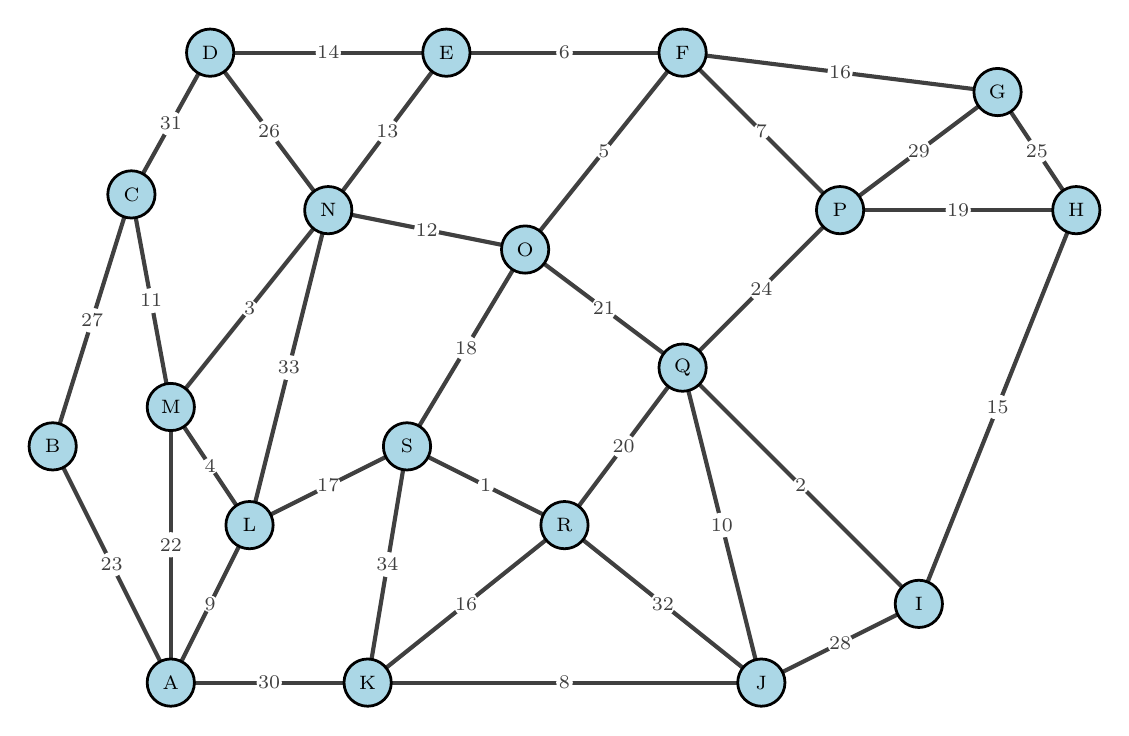
\begin{tikzpicture}
    \Vertex[x=1.5, y=0, label=A]{A}
    \Vertex[x=0, y=3, label=B]{B}
    \Vertex[x=1, y=6.2, label=C]{C}
    \Vertex[x=2, y=8, label=D]{D}
    \Vertex[x=5, y=8, label=E]{E}
    \Vertex[x=8, y=8, label=F]{F}
    \Vertex[x=12, y=7.5, label=G]{G}
    \Vertex[x=13, y=6, label=H]{H}
    \Vertex[x=11, y=1, label=I]{I}
    \Vertex[x=9, y=0, label=J]{J}
    \Vertex[x=4, y=0, label=K]{K}
    \Vertex[x=2.5, y=2, label=L]{L}
    \Vertex[x=1.5, y=3.5, label=M]{M}
    \Vertex[x=3.5, y=6, label=N]{N}
    \Vertex[x=6, y=5.5, label=O]{O}
    \Vertex[x=10, y=6, label=P]{P}
    \Vertex[x=8, y=4, label=Q]{Q}
    \Vertex[x=6.5, y=2, label=R]{R}
    \Vertex[x=4.5, y=3, label=S]{S}
    
    \Edge[label=1](R)(S)
    \Edge[label=2](Q)(I)
    \Edge[label=3](M)(N)
    \Edge[label=4](L)(M)
    \Edge[label=5](O)(F)
    \Edge[label=6](E)(F)
    \Edge[label=7](P)(F)
    \Edge[label=8](J)(K)
    \Edge[label=9](A)(L)
    \Edge[label=10](Q)(J)
    \Edge[label=11](M)(C)
    \Edge[label=12](N)(O)
    \Edge[label=13](N)(E)
    \Edge[label=14](D)(E)
    \Edge[label=15](H)(I)
    \Edge[label=16](F)(G)
    \Edge[label=16](K)(R)
    \Edge[label=17](L)(S)
    \Edge[label=18](S)(O)
    \Edge[label=19](P)(H)
    \Edge[label=20](R)(Q)
    \Edge[label=21](Q)(O)
    \Edge[label=22](A)(M)
    \Edge[label=23](A)(B)
    \Edge[label=24](Q)(P)
    \Edge[label=25](G)(H)
    \Edge[label=26](N)(D)
    \Edge[label=27](B)(C)
    \Edge[label=28](I)(J)
    \Edge[label=29](P)(G)
    \Edge[label=30](K)(A)
    \Edge[label=31](C)(D)
    \Edge[label=33](L)(N)
    \Edge[label=32](J)(R)
    \Edge[label=34](K)(S)
\end{tikzpicture}


\subsection*{Minimum Spanning Tree}
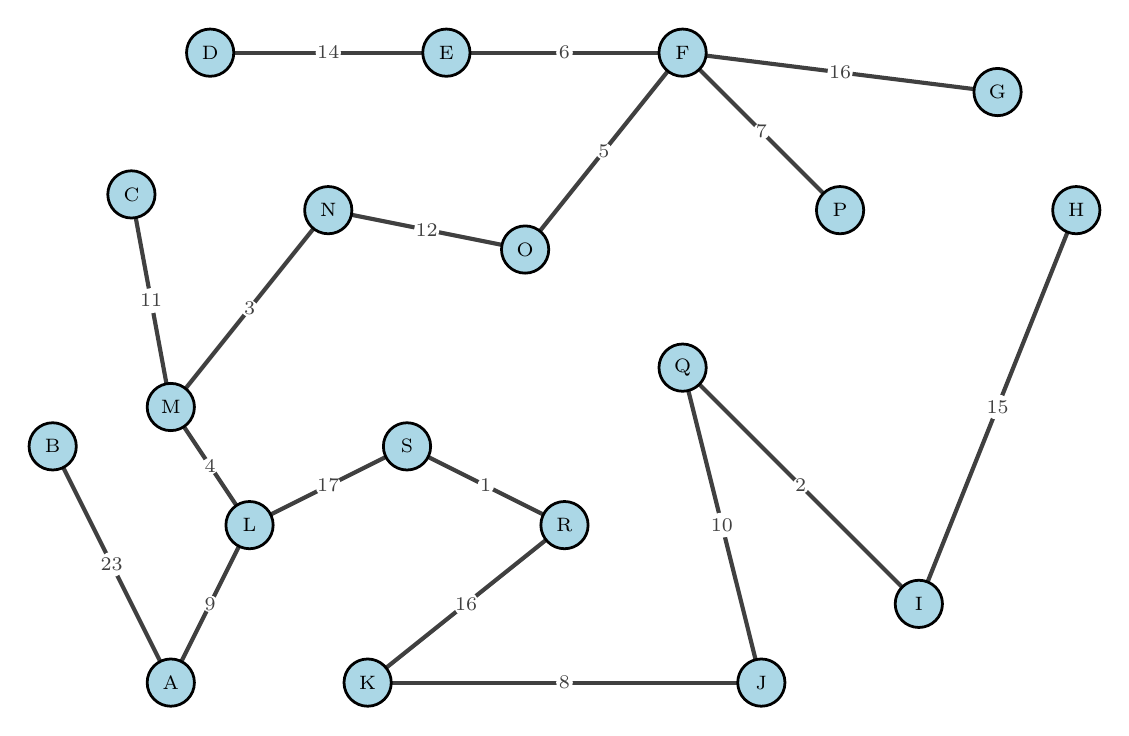
\begin{tikzpicture}
    \Vertex[x=1.5, y=0, label=A]{A}
    \Vertex[x=0, y=3, label=B]{B}
    \Vertex[x=1, y=6.2, label=C]{C}
    \Vertex[x=2, y=8, label=D]{D}
    \Vertex[x=5, y=8, label=E]{E}
    \Vertex[x=8, y=8, label=F]{F}
    \Vertex[x=12, y=7.5, label=G]{G}
    \Vertex[x=13, y=6, label=H]{H}
    \Vertex[x=11, y=1, label=I]{I}
    \Vertex[x=9, y=0, label=J]{J}
    \Vertex[x=4, y=0, label=K]{K}
    \Vertex[x=2.5, y=2, label=L]{L}
    \Vertex[x=1.5, y=3.5, label=M]{M}
    \Vertex[x=3.5, y=6, label=N]{N}
    \Vertex[x=6, y=5.5, label=O]{O}
    \Vertex[x=10, y=6, label=P]{P}
    \Vertex[x=8, y=4, label=Q]{Q}
    \Vertex[x=6.5, y=2, label=R]{R}
    \Vertex[x=4.5, y=3, label=S]{S}
    
    \Edge[label=1](R)(S)
    \Edge[label=2](Q)(I)
    \Edge[label=3](M)(N)
    \Edge[label=4](L)(M)
    \Edge[label=5](O)(F)
    \Edge[label=6](E)(F)
    \Edge[label=7](P)(F)
    \Edge[label=8](J)(K)
    \Edge[label=9](A)(L)
    \Edge[label=10](Q)(J)
    \Edge[label=11](M)(C)
    \Edge[label=12](N)(O)
    \Edge[label=14](D)(E)
    \Edge[label=15](H)(I)
    \Edge[label=16](F)(G)
    \Edge[label=16](K)(R)
    \Edge[label=17](L)(S)
    \Edge[label=23](A)(B)
\end{tikzpicture}

\end{document}